% =====================================================================
% Appendix A -- Additional experimental details and results
% Tables generated by scripts/make_appendix_tables.py (run by scripts/run_all.py).
% Every paragraph marked CLAUDE-DRAFT is to be rewritten by the author.
% =====================================================================

\chapter{Additional Experimental Details and Results}
\label{app:results}

% CLAUDE-DRAFT
This appendix complements \cref{chap:experiments}.
\Cref{sec:app-volumes} lists the volumes of the few-shot training sets and of the test sets, \cref{sec:app-params} the settings and parameters of all runs, \cref{sec:app-additional} the additional evaluations, \cref{sec:exp-components} the weight ensemble and the gradient scaling, and \cref{sec:app-matrices} gives the evaluation matrix of every run reported in \cref{chap:experiments}, from which all metrics and all per-task values quoted there are computed.
\Cref{sec:app-shared-loss} shows the training loss of the first two tasks of shared LoRA.

\section{Training and Test Volumes}
\label{sec:app-volumes}

% CLAUDE-DRAFT
This section belongs to \cref{sec:data-splits,subsec:exp-data}.
\Cref{tab:app-volumes} lists the SKM-TEA volumes of the few-shot training sets and the test volumes of both datasets.
The few-shot sets are taken from the training logs of the runs: every run with the same number of volumes~$k$ used the same set for all six tasks, and the sets are nested.
The test volumes are the same in every run.

\begin{table}[tb]
\centering
% CLAUDE-DRAFT
\caption[Few-shot training volumes and test volumes]{Few-shot training volumes and test volumes. SKM-TEA volumes by their identifier, AeroPath volumes by their number. The full training split contains 108 SKM-TEA volumes.}
\label{tab:app-volumes}
% Generated by scripts/make_appendix_tables.py. Do not edit.
\small
\begin{tabularx}{\linewidth}{@{}l>{\raggedright\arraybackslash}X@{}}
\toprule
Set & Volumes \\
\midrule
SKM-TEA training, $k = 5$ & MTR\_038, MTR\_074, MTR\_097, MTR\_201, MTR\_225 \\
SKM-TEA training, $k = 10$ & the 5 volumes above and MTR\_118, MTR\_154, MTR\_188, MTR\_207, MTR\_219 \\
SKM-TEA training, $k = 20$ & the 10 volumes above and MTR\_001, MTR\_037, MTR\_056, MTR\_120, MTR\_156, MTR\_167, MTR\_179, MTR\_209, MTR\_224, MTR\_243 \\
SKM-TEA test (24 volumes) & MTR\_005, MTR\_015, MTR\_016, MTR\_018, MTR\_045, MTR\_046, MTR\_049, MTR\_052, MTR\_066, MTR\_079, MTR\_098, MTR\_104, MTR\_105, MTR\_107, MTR\_110, MTR\_115, MTR\_129, MTR\_130, MTR\_190, MTR\_191, MTR\_199, MTR\_215, MTR\_227, MTR\_248 \\
AeroPath test (4 volumes) & 1, 3, 6, 12 \\
\bottomrule
\end{tabularx}

\end{table}

\section{Training and Strategy Parameters}
\label{sec:app-params}

% CLAUDE-DRAFT
This section belongs to \cref{subsec:exp-config}.
\Cref{tab:app-hparams} lists the training and evaluation settings that all runs share, and \cref{tab:app-strategy-params} the parameters of each strategy.
Both tables are generated from the configuration files of the runs; the few values that are defaults of the code are checked against the code by the same script.

% CLAUDE-DRAFT
The software environment comprises PyTorch 2.8.0 with CUDA 12.6 and cuDNN 9.10.2, MONAI 1.5.2, nnU-Net 2.7.0, Transformers 4.57.6, NumPy 2.4.3 and NiBabel 5.4.2.
% source: author's pip list / torch.version on the HPC environment "voxtell", 2026-10-22
The software versions were not logged per run but read from the environment after training, and the code version was recorded only for the reruns.\todo{defense: software versions not logged per run; read from the environment on 2026-10-22 (moved from Sec. 6.1.2, then Sec. 7.3)}
% source: thesis_notes.md §3 (code version per run not recorded; D32)
The training logs of the distillation-based strategy record only its total loss, so the contribution of the distillation term cannot be determined.\todo{defense: distillation term not logged separately (moved from Sec. 6.2, then Sec. 7.3)}

% CLAUDE-DRAFT
Runs that reached the 24-hour limit of a job were continued from their last checkpoint.
Continuing at a task boundary did not change the results: the reruns of sequential fine-tuning with 5, 10 and 20 volumes and in the reverse order reproduce every entry of the evaluation matrices of the earlier runs with the same configuration.
Five runs of the comparison of the strategies and of the few-shot experiment were continued inside a task; from that point on, they draw training samples and patches in a different order, so they cannot be reproduced exactly from their configuration.
% source: thesis_notes.md §2 Reproducibility (2026-10-26): best_validation matrices of the reruns vs the earlier runs (max |diff| 0); resumes inside a task in SLURM logs 1848498, 1848499, 1848503, 1849216, 1850677
% source: code/src/training/utils.py (use_deterministic_algorithms with warn_only=True)

\begin{table}[tb]
\centering
% CLAUDE-DRAFT
\caption[Training and evaluation settings shared by all runs]{Training and evaluation settings shared by all runs (\cref{sec:method-setting-protocol,sec:method-adaptation}).}
\label{tab:app-hparams}
% Generated by scripts/make_setup_tables.py. Do not edit.
\small
\begin{tabular}{@{}ll>{\raggedright\arraybackslash}p{6.4cm}@{}}
\toprule
Setting & Symbol & Value \\
\midrule
Optimiser &  & SGD, Nesterov \\
Initial learning rate & $\eta_0$ & $10^{-4}$ \\
Momentum & $\mu$ & $0.99$ \\
Weight decay & $\omega$ & $3 \cdot 10^{-5}$ \\
Learning-rate schedule &  & linear (polynomial, exponent 1), per iteration, restarted for every task \\
Epochs per task & $E$ & 10; 216 in the equal-updates runs (validation every 24 epochs) \\
Batch size &  & 1 \\
Patch size (voxels) &  & $192 \times 192 \times 192$ \\
Foreground-centred patches & $\pi_{\mathrm{fg}}$ & 0.85 \\
Loss & $\mathcal{L}_{\mathrm{seg}}$ & binary cross-entropy + soft Dice (smoothing $10^{-5}$), weights 1:1 \\
Deep supervision &  & off \\
Dropout in the prompt decoder &  & 0.1; inactive in the prompt-tuning strategy, 0 on the attention weights in the LoRA strategies \\
Data augmentation &  & none \\
Random seed (training, split) &  & 42, 42 \\
Sliding-window step &  & 0.5 of the patch size \\
Gaussian weighting &  & standard deviation 1/8 of the patch size \\
Probability threshold &  & 0.5 \\
\bottomrule
\end{tabular}

\end{table}

\begin{table}[tbp]
\centering
% CLAUDE-DRAFT
\caption[Parameters of the strategies]{Parameters of the strategies (\cref{sec:method-strategies}). Sequential fine-tuning has no parameters of its own. Bold: rank used in the comparison of the strategies; scaling factor $\gamma_r = \alpha/\sqrt{r}$ listed per rank. The weight ensemble of the distillation-based strategy is reported as an additional evaluation; the run of the prompt-tuning strategy without gradient scaling has the same parameters with the scale inactive.}
\label{tab:app-strategy-params}
% Generated by scripts/make_setup_tables.py. Do not edit.
\small
\begin{tabular}{@{}>{\raggedright\arraybackslash}p{2.6cm}ll>{\raggedright\arraybackslash}p{4.4cm}@{}}
\toprule
Strategy & Parameter & Symbol & Value \\
\midrule
Task-specific LoRA & Rank & $r$ & \textbf{4}, 8 \\
 & Scaling constant & $\alpha$ & 16 \\
 & Scaling factor & $\gamma_r$ & 8, 5.66 \\
 & Dropout (low-rank path) &  & 0.05 \\
 & Adapted projections &  & $\mat{W}_q, \mat{W}_v$, cross-attention \\
\addlinespace
Shared LoRA & Rank & $r$ & 4, 32, 128, 256, 512, \textbf{1024}, 2048 \\
 & Scaling constant & $\alpha$ & 32 \\
 & Scaling factor & $\gamma_r$ & 16, 5.66, 2.83, 2, 1.41, 1, 0.71 \\
 & Dropout (low-rank path) &  & 0.1 \\
 & Adapted projections &  & $\mat{W}_q, \mat{W}_v$, cross-attention \\
\addlinespace
Shared LoRA + replay & Rank (otherwise as shared LoRA) & $r$ & 1024 \\
 & Replay fraction & $\rho$ & 0.1 \\
 & Maximum memory size & $M_{\max}$ & 200 \\
\addlinespace
Distillation-based & Distillation weight & $\lambda$ & $0.01$ \\
 & Ensemble interval (iterations) & $I_{\mathrm{we}}$ & 10 \\
\addlinespace
Prompt tuning & Learned prompt tokens per layer & $m$ & 2 \\
 & Prompted decoder layers & $L_p$ & 3 \\
 & Gradient-scale lower bound &  & 0.25 \\
\bottomrule
\end{tabular}

\end{table}

\section{Additional Evaluations}
\label{sec:app-additional}

% CLAUDE-DRAFT
This section belongs to \cref{sec:exp-main}; \cref{sec:exp-components} uses its metrics.
\Cref{tab:ch6_components} gives the metrics of the additional evaluations; the parameters after the last epoch of the same runs are in \cref{tab:ch6_main}.

\begin{table}[tb]
\centering
% CLAUDE-DRAFT
\caption[Additional evaluations]{Additional evaluations (full training split, original task order, one run each). Best validation: parameters with the lowest validation loss; weight ensemble: the weight ensemble of the distillation-based strategy (\cref{sec:method-adaptation,subsec:method-distillation}). No scaling: the earlier run of the prompt-tuning strategy with the per-task gradient scale inactive, evaluated only at the checkpoint with the lowest validation loss (\cref{subsec:method-prompt}). Mean \gls{dsc}; $\uparrow$/$\downarrow$: higher/lower is better.}
\label{tab:ch6_components}
% Generated by scripts/make_results_tables.py from thesis/tables/cl_metrics.csv. Do not edit.
\small\setlength{\tabcolsep}{3pt}
\begin{tabular}{llrrrrr}
\toprule
Strategy & Evaluation & Adapt.\,$\uparrow$ & Forg.\,$\downarrow$ & Ctrl.\ drop\,$\downarrow$ & Final\,$\uparrow$ & Transf.\,$\uparrow$ \\
\midrule
Seq. fine-tuning & last epoch & 0.781 & 0.782 & 0.979 & 0.130 & 0.001 \\
Seq. fine-tuning & best validation & 0.723 & 0.712 & 0.979 & 0.130 & 0.001 \\
\addlinespace
Prompt tuning & last epoch & 0.580 & 0.510 & 0.865 & 0.155 & 0.043 \\
Prompt tuning & best validation & 0.576 & 0.505 & 0.863 & 0.155 & 0.039 \\
\addlinespace
Prompt tuning (no scaling) & best validation & 0.608 & 0.568 & 0.979 & 0.135 & 0.043 \\
\addlinespace
Distillation-based & last epoch & 0.747 & 0.734 & 0.979 & 0.135 & 0.002 \\
Distillation-based & best validation & 0.745 & 0.732 & 0.979 & 0.135 & 0.002 \\
Distillation-based & weight ensemble & 0.376 & 0.354 & 0.979 & 0.124 & 0.007 \\
\midrule
Pretrained model &  & 0.114 & 0.000 & 0.000 & 0.114 & 0.137 \\
\bottomrule
\end{tabular}

\end{table}

\section{Weight Ensemble and Gradient Scaling}
\label{sec:exp-components}
% Split from Sec. 6.2 on 2026-11-02 (author decision; reverses the 2026-10-24 decision, thesis_notes.md section 1).
% Narrowed 2026-11-04 (author decision): replay moved to Sec. 6.2; title changed from "Components of the Strategies"; label kept.
% Moved from Ch. 6 (Sec. 6.7) to App. A on 2026-11-05 (author decision: weak evidence, appendix tables, page budget); Sec. 6.2 points here.
% CLAUDE-DRAFT
This section belongs to \cref{sec:exp-main}.
It reports how the weight ensemble of the distillation-based strategy and the per-task gradient scaling of the prompt-tuning strategy affect adaptation and forgetting.
Both components are adopted from the published methods, ZSCL and CPE-CLIP, and each is compared with the same strategy without it.
The weight ensemble is evaluated in the same run as the student, and gradient scaling is compared against an earlier run without it.
\Cref{tab:ch6_components} in \cref{sec:app-additional} gives the metrics of these evaluations, \cref{tab:ch6_main} those after the last epoch, and \cref{tab:app-we-matrix} the evaluation matrix of the weight ensemble.

% CLAUDE-DRAFT
The weight ensemble of the distillation-based strategy halved the Adaptation of the student, from 0.747 to 0.376, lowered the Final Performance by 0.011 $[0.007, 0.017]$ and left the control-task drop unchanged.
Its Final Forgetting of 0.354, against 0.734 for the student, is lower only because the ensemble learned less in the first place.
On the diagonal of its evaluation matrix (\cref{tab:app-we-matrix}), the \gls{dsc} fell from 0.83 on the first task to 0.22 on the fourth and to 0.00 on the last two.
A possible explanation follows from the definition of the ensemble as the equally weighted mean of $\theta_0$ and all snapshots, with 100 snapshots per task (\cref{subsec:method-distillation}).
After task~$t$, the snapshots of that task make up only about $1/t$ of the ensemble, so it follows each later task less.
The ensemble also could not protect the control task, because the student had already lost it after the first task (\gls{dsc} 0.00), and the ensemble averages such states.
Our ensemble differs from that of ZSCL in its update interval, in not being restarted at each task and in the distillation without a reference dataset (\cref{subsec:method-distillation}), so these results hold for our configuration only.\todo{defense: weight ensemble not restarted per task and not carried forward (unlike ZSCL's code), interval of 10, no reference dataset; explanation of the low Adaptation (weights of late snapshots) not tested}
% source: cl_differences.csv, exp_20261022_171452_65011743:weight_ensemble - exp_20261022_171452_65011743; diagonal of evaluations/weight_ensemble/eval_matrix.csv; 100 ensemble updates per task (10 per epoch, thesis_notes.md §2)

{\captionsetup{list=no}% Generated by scripts/make_appendix_tables.py. Do not edit.
\noindent\begin{minipage}{\linewidth}\centering\small
\captionof{table}{Evaluation matrix of the weight ensemble of the distillation-based strategy (full training split, original task order); run \texttt{exp\_20261022\_171452\_65011743}.}\label{tab:app-we-matrix}
\setlength{\tabcolsep}{5pt}
\begin{tabular}{lrrrrrrr}
\toprule
Task & Pre & LT & MT & Fe & Pa & MM & LM \\
\midrule
LT & 0.000 & \textbf{0.828} & 0.002 & 0.003 & 0.001 & 0.001 & 0.000 \\
MT & 0.000 & 0.001 & \textbf{0.690} & 0.300 & 0.095 & 0.033 & 0.010 \\
Fe & 0.684 & 0.002 & 0.009 & \textbf{0.514} & 0.615 & 0.415 & 0.286 \\
Pa & 0.000 & 0.000 & 0.000 & 0.069 & \textbf{0.219} & 0.372 & 0.446 \\
MM & 0.000 & 0.000 & 0.003 & 0.006 & 0.005 & \textbf{0.002} & 0.000 \\
LM & 0.000 & 0.009 & 0.000 & 0.000 & 0.000 & 0.000 & \textbf{0.000} \\
\midrule
Ctrl & 0.979 & 0.002 & 0.000 & 0.000 & 0.000 & 0.000 & 0.000 \\
\bottomrule
\end{tabular}
\end{minipage}
\par\bigskip
}

% CLAUDE-DRAFT
The per-task gradient scaling of the prompt-tuning strategy lowered its forgetting at a small cost in Adaptation.
Both runs are compared at the checkpoint with the lowest validation loss, because the run without scaling was evaluated only there.
With scaling, Final Forgetting was 0.063 lower, the control-task drop 0.117 lower and Final Performance 0.020 higher $[0.014, 0.025]$, at an Adaptation lower by 0.032 $[0.025, 0.040]$.
Without scaling, the \gls{dsc} on the lung fell to 0.02 after the second task and to 0.00 at the end.
With scaling, it stayed between 0.04 and 0.23 from the first task on.
Scaling down the gradients in later tasks thus traded a little adaptation for retention, but it did not keep the control task.
% source: cl_differences.csv, exp_20261022_180923_7bcbb6cc:best_validation - exp_20260816_161201_b39ea60e; control rows of both runs (best_validation/eval_matrix.csv: 0.042-0.226, checked 2026-11-04)

% Conclusion suggested by Claude and accepted by the author (2026-11-04), replacing that of 2026-11-02 after replay moved to Sec. 6.2.
% CLAUDE-DRAFT
Of the two components, only the gradient scaling moved its strategy towards retention, at a small cost in Adaptation.
Neither kept the control task.
The student of the distillation-based strategy had already lost it after the first task, and the prompt-tuning strategy lost most of it with scaling as well.
Both components differ from their published form (\cref{sec:method-strategies}), and each was tested in one run and in the original task order, so these results hold for our configuration only.\todo{defense: components tested once each, one strategy, one task order; scaling compared at best-validation checkpoints against an earlier run}

\section{Evaluation Matrices of All Runs}
\label{sec:app-matrices}

% CLAUDE-DRAFT
This section belongs to \cref{chap:experiments}.
For every reported run, the table gives the mean \gls{dsc} on the test volumes of each task (rows, in training order) after each stage (columns): \emph{Pre.} is the pretrained model, and the following columns are the stages after training on the task named in the header.
The diagonal entries, right after a task is trained, are set in bold; the last row is the control task.
Task abbreviations: LT lateral tibial cartilage, MT medial tibial cartilage, Fe femoral cartilage, Pa patellar cartilage, MM medial meniscus, LM lateral meniscus, Ctrl control task (lung in AeroPath).
The runs are grouped by the experiment in which they first appear in \cref{tab:ch6_experiments}; a run that belongs to several experiments is listed once, and the prompt-tuning run without gradient scaling (\cref{sec:exp-components}), which is not in that table, is listed last.
Joint fine-tuning has a single stage, \emph{Joint}, after which all six structures are evaluated.
All matrices are computed with the parameters after the last epoch, except that of the prompt-tuning run without gradient scaling, which was evaluated only at the checkpoint with the lowest validation loss (\cref{sec:exp-components}).

% Generated by scripts/make_appendix_tables.py. Do not edit.
\captionsetup{list=no}
\subsection*{Comparison of the strategies}
\noindent\begin{minipage}{\linewidth}\centering\small
\captionof{table}{Evaluation matrix: Sequential fine-tuning (full training split, original task order); run \texttt{exp\_20260816\_155351\_cfa776e7}.}
\setlength{\tabcolsep}{5pt}
\begin{tabular}{lrrrrrrr}
\toprule
Task & Pre. & LT & MT & Fe & Pa & MM & LM \\
\midrule
LT & 0.000 & \textbf{0.712} & 0.000 & 0.001 & 0.004 & 0.000 & 0.019 \\
MT & 0.000 & 0.000 & \textbf{0.837} & 0.002 & 0.000 & 0.011 & 0.000 \\
Fe & 0.684 & 0.001 & 0.001 & \textbf{0.841} & 0.271 & 0.006 & 0.006 \\
Pa & 0.000 & 0.000 & 0.000 & 0.004 & \textbf{0.424} & 0.002 & 0.038 \\
MM & 0.000 & 0.000 & 0.009 & 0.001 & 0.000 & \textbf{0.779} & 0.013 \\
LM & 0.000 & 0.007 & 0.000 & 0.001 & 0.000 & 0.000 & \textbf{0.705} \\
\midrule
Ctrl & 0.979 & 0.002 & 0.000 & 0.000 & 0.000 & 0.000 & 0.000 \\
\bottomrule
\end{tabular}
\end{minipage}
\par\bigskip
\noindent\begin{minipage}{\linewidth}\centering\small
\captionof{table}{Evaluation matrix: Task-specific LoRA ($r = 4$, full training split, original task order); run \texttt{exp\_20260816\_155157\_668e608d}.}
\setlength{\tabcolsep}{5pt}
\begin{tabular}{lrrrrrrr}
\toprule
Task & Pre. & LT & MT & Fe & Pa & MM & LM \\
\midrule
LT & 0.000 & \textbf{0.635} & 0.635 & 0.635 & 0.635 & 0.635 & 0.635 \\
MT & 0.000 & 0.163 & \textbf{0.527} & 0.527 & 0.527 & 0.527 & 0.527 \\
Fe & 0.684 & 0.440 & 0.470 & \textbf{0.774} & 0.774 & 0.774 & 0.774 \\
Pa & 0.000 & 0.002 & 0.002 & 0.000 & \textbf{0.000} & 0.000 & 0.000 \\
MM & 0.000 & 0.012 & 0.042 & 0.000 & 0.000 & \textbf{0.572} & 0.572 \\
LM & 0.000 & 0.033 & 0.006 & 0.000 & 0.000 & 0.020 & \textbf{0.401} \\
\midrule
Ctrl & 0.979 & 0.979 & 0.979 & 0.979 & 0.979 & 0.979 & 0.979 \\
\bottomrule
\end{tabular}
\end{minipage}
\par\bigskip
\noindent\begin{minipage}{\linewidth}\centering\small
\captionof{table}{Evaluation matrix: Shared LoRA ($r = 1024$, full training split, original task order); run \texttt{exp\_20260926\_095539\_90e8b4e6}.}
\setlength{\tabcolsep}{5pt}
\begin{tabular}{lrrrrrrr}
\toprule
Task & Pre. & LT & MT & Fe & Pa & MM & LM \\
\midrule
LT & 0.000 & \textbf{0.294} & 0.311 & 0.174 & 0.156 & 0.216 & 0.025 \\
MT & 0.000 & 0.185 & \textbf{0.490} & 0.326 & 0.165 & 0.355 & 0.018 \\
Fe & 0.684 & 0.648 & 0.550 & \textbf{0.719} & 0.609 & 0.644 & 0.555 \\
Pa & 0.000 & 0.024 & 0.004 & 0.008 & \textbf{0.443} & 0.291 & 0.039 \\
MM & 0.000 & 0.037 & 0.061 & 0.030 & 0.066 & \textbf{0.477} & 0.357 \\
LM & 0.000 & 0.020 & 0.026 & 0.008 & 0.011 & 0.071 & \textbf{0.402} \\
\midrule
Ctrl & 0.979 & 0.980 & 0.975 & 0.976 & 0.974 & 0.955 & 0.742 \\
\bottomrule
\end{tabular}
\end{minipage}
\par\bigskip
\noindent\begin{minipage}{\linewidth}\centering\small
\captionof{table}{Evaluation matrix: Prompt-tuning strategy (full training split, original task order); run \texttt{exp\_20260816\_161201\_b39ea60e}.}
\setlength{\tabcolsep}{5pt}
\begin{tabular}{lrrrrrrr}
\toprule
Task & Pre. & LT & MT & Fe & Pa & MM & LM \\
\midrule
LT & 0.000 & \textbf{0.707} & 0.364 & 0.109 & 0.055 & 0.164 & 0.017 \\
MT & 0.000 & 0.102 & \textbf{0.549} & 0.119 & 0.025 & 0.090 & 0.001 \\
Fe & 0.684 & 0.088 & 0.033 & \textbf{0.777} & 0.408 & 0.006 & 0.001 \\
Pa & 0.000 & 0.002 & 0.000 & 0.015 & \textbf{0.434} & 0.033 & 0.002 \\
MM & 0.000 & 0.008 & 0.019 & 0.012 & 0.007 & \textbf{0.555} & 0.162 \\
LM & 0.000 & 0.009 & 0.002 & 0.005 & 0.001 & 0.166 & \textbf{0.629} \\
\midrule
Ctrl & 0.979 & 0.108 & 0.019 & 0.060 & 0.001 & 0.002 & 0.000 \\
\bottomrule
\end{tabular}
\end{minipage}
\par\bigskip
\noindent\begin{minipage}{\linewidth}\centering\small
\captionof{table}{Evaluation matrix: Distillation-based strategy (full training split, original task order); run \texttt{exp\_20260924\_204124\_7ce6758c}.}
\setlength{\tabcolsep}{5pt}
\begin{tabular}{lrrrrrrr}
\toprule
Task & Pre. & LT & MT & Fe & Pa & MM & LM \\
\midrule
LT & 0.000 & \textbf{0.841} & 0.001 & 0.001 & 0.005 & 0.000 & 0.009 \\
MT & 0.000 & 0.000 & \textbf{0.821} & 0.004 & 0.003 & 0.010 & 0.000 \\
Fe & 0.684 & 0.001 & 0.001 & \textbf{0.819} & 0.248 & 0.006 & 0.004 \\
Pa & 0.000 & 0.000 & 0.000 & 0.011 & \textbf{0.477} & 0.000 & 0.000 \\
MM & 0.000 & 0.000 & 0.012 & 0.001 & 0.000 & \textbf{0.726} & 0.013 \\
LM & 0.000 & 0.007 & 0.000 & 0.002 & 0.000 & 0.004 & \textbf{0.780} \\
\midrule
Ctrl & 0.979 & 0.002 & 0.000 & 0.002 & 0.002 & 0.000 & 0.000 \\
\bottomrule
\end{tabular}
\end{minipage}
\par\bigskip
\subsection*{LoRA rank}
\noindent\begin{minipage}{\linewidth}\centering\small
\captionof{table}{Evaluation matrix: Task-specific LoRA ($r = 8$, full training split, original task order); run \texttt{exp\_20260822\_110320\_530ca92a}.}
\setlength{\tabcolsep}{5pt}
\begin{tabular}{lrrrrrrr}
\toprule
Task & Pre. & LT & MT & Fe & Pa & MM & LM \\
\midrule
LT & 0.000 & \textbf{0.515} & 0.515 & 0.515 & 0.515 & 0.515 & 0.515 \\
MT & 0.000 & 0.273 & \textbf{0.516} & 0.516 & 0.516 & 0.516 & 0.516 \\
Fe & 0.684 & 0.601 & 0.488 & \textbf{0.748} & 0.748 & 0.748 & 0.748 \\
Pa & 0.000 & 0.006 & 0.002 & 0.000 & \textbf{0.000} & 0.000 & 0.000 \\
MM & 0.000 & 0.021 & 0.077 & 0.000 & 0.000 & \textbf{0.526} & 0.526 \\
LM & 0.000 & 0.040 & 0.008 & 0.000 & 0.000 & 0.033 & \textbf{0.118} \\
\midrule
Ctrl & 0.979 & 0.979 & 0.979 & 0.979 & 0.979 & 0.979 & 0.979 \\
\bottomrule
\end{tabular}
\end{minipage}
\par\bigskip
\noindent\begin{minipage}{\linewidth}\centering\small
\captionof{table}{Evaluation matrix: Shared LoRA ($r = 4$, full training split, original task order); run \texttt{exp\_20260924\_202757\_88afb75d}.}
\setlength{\tabcolsep}{5pt}
\begin{tabular}{lrrrrrrr}
\toprule
Task & Pre. & LT & MT & Fe & Pa & MM & LM \\
\midrule
LT & 0.000 & \textbf{0.693} & 0.380 & 0.022 & 0.051 & 0.022 & 0.005 \\
MT & 0.000 & 0.104 & \textbf{0.520} & 0.065 & 0.004 & 0.053 & 0.001 \\
Fe & 0.684 & 0.053 & 0.096 & \textbf{0.783} & 0.547 & 0.069 & 0.004 \\
Pa & 0.000 & 0.000 & 0.000 & 0.031 & \textbf{0.510} & 0.005 & 0.000 \\
MM & 0.000 & 0.002 & 0.011 & 0.039 & 0.012 & \textbf{0.581} & 0.348 \\
LM & 0.000 & 0.011 & 0.001 & 0.021 & 0.001 & 0.062 & \textbf{0.554} \\
\midrule
Ctrl & 0.979 & 0.004 & 0.001 & 0.330 & 0.014 & 0.226 & 0.001 \\
\bottomrule
\end{tabular}
\end{minipage}
\par\bigskip
\noindent\begin{minipage}{\linewidth}\centering\small
\captionof{table}{Evaluation matrix: Shared LoRA ($r = 32$, full training split, original task order); run \texttt{exp\_20260926\_095635\_1dd1adb4}.}
\setlength{\tabcolsep}{5pt}
\begin{tabular}{lrrrrrrr}
\toprule
Task & Pre. & LT & MT & Fe & Pa & MM & LM \\
\midrule
LT & 0.000 & \textbf{0.650} & 0.427 & 0.140 & 0.100 & 0.195 & 0.010 \\
MT & 0.000 & 0.175 & \textbf{0.515} & 0.158 & 0.038 & 0.201 & 0.004 \\
Fe & 0.684 & 0.458 & 0.183 & \textbf{0.751} & 0.504 & 0.439 & 0.018 \\
Pa & 0.000 & 0.003 & 0.000 & 0.014 & \textbf{0.492} & 0.179 & 0.016 \\
MM & 0.000 & 0.024 & 0.025 & 0.082 & 0.029 & \textbf{0.517} & 0.381 \\
LM & 0.000 & 0.031 & 0.002 & 0.012 & 0.003 & 0.103 & \textbf{0.493} \\
\midrule
Ctrl & 0.979 & 0.708 & 0.193 & 0.880 & 0.106 & 0.080 & 0.001 \\
\bottomrule
\end{tabular}
\end{minipage}
\par\bigskip
\noindent\begin{minipage}{\linewidth}\centering\small
\captionof{table}{Evaluation matrix: Shared LoRA ($r = 128$, full training split, original task order); run \texttt{exp\_20260816\_124851\_bc388139}.}
\setlength{\tabcolsep}{5pt}
\begin{tabular}{lrrrrrrr}
\toprule
Task & Pre. & LT & MT & Fe & Pa & MM & LM \\
\midrule
LT & 0.000 & \textbf{0.453} & 0.316 & 0.102 & 0.111 & 0.242 & 0.015 \\
MT & 0.000 & 0.241 & \textbf{0.531} & 0.164 & 0.058 & 0.289 & 0.010 \\
Fe & 0.684 & 0.633 & 0.417 & \textbf{0.732} & 0.630 & 0.639 & 0.358 \\
Pa & 0.000 & 0.014 & 0.001 & 0.008 & \textbf{0.484} & 0.230 & 0.024 \\
MM & 0.000 & 0.034 & 0.044 & 0.071 & 0.034 & \textbf{0.490} & 0.363 \\
LM & 0.000 & 0.029 & 0.009 & 0.002 & 0.004 & 0.101 & \textbf{0.455} \\
\midrule
Ctrl & 0.979 & 0.969 & 0.791 & 0.937 & 0.672 & 0.434 & 0.022 \\
\bottomrule
\end{tabular}
\end{minipage}
\par\bigskip
\noindent\begin{minipage}{\linewidth}\centering\small
\captionof{table}{Evaluation matrix: Shared LoRA ($r = 256$, full training split, original task order); run \texttt{exp\_20260817\_172554\_da49178a}.}
\setlength{\tabcolsep}{5pt}
\begin{tabular}{lrrrrrrr}
\toprule
Task & Pre. & LT & MT & Fe & Pa & MM & LM \\
\midrule
LT & 0.000 & \textbf{0.361} & 0.309 & 0.142 & 0.121 & 0.247 & 0.014 \\
MT & 0.000 & 0.223 & \textbf{0.522} & 0.223 & 0.085 & 0.343 & 0.012 \\
Fe & 0.684 & 0.646 & 0.468 & \textbf{0.726} & 0.634 & 0.664 & 0.478 \\
Pa & 0.000 & 0.023 & 0.002 & 0.008 & \textbf{0.478} & 0.243 & 0.014 \\
MM & 0.000 & 0.042 & 0.056 & 0.053 & 0.045 & \textbf{0.489} & 0.373 \\
LM & 0.000 & 0.026 & 0.014 & 0.004 & 0.005 & 0.089 & \textbf{0.443} \\
\midrule
Ctrl & 0.979 & 0.979 & 0.945 & 0.968 & 0.918 & 0.772 & 0.148 \\
\bottomrule
\end{tabular}
\end{minipage}
\par\bigskip
\noindent\begin{minipage}{\linewidth}\centering\small
\captionof{table}{Evaluation matrix: Shared LoRA ($r = 512$, full training split, original task order); run \texttt{exp\_20260924\_163047\_f4aa9c98}.}
\setlength{\tabcolsep}{5pt}
\begin{tabular}{lrrrrrrr}
\toprule
Task & Pre. & LT & MT & Fe & Pa & MM & LM \\
\midrule
LT & 0.000 & \textbf{0.310} & 0.290 & 0.137 & 0.143 & 0.192 & 0.020 \\
MT & 0.000 & 0.201 & \textbf{0.511} & 0.264 & 0.145 & 0.321 & 0.014 \\
Fe & 0.684 & 0.647 & 0.516 & \textbf{0.721} & 0.619 & 0.640 & 0.537 \\
Pa & 0.000 & 0.029 & 0.003 & 0.010 & \textbf{0.461} & 0.251 & 0.020 \\
MM & 0.000 & 0.042 & 0.058 & 0.038 & 0.061 & \textbf{0.494} & 0.361 \\
LM & 0.000 & 0.022 & 0.023 & 0.006 & 0.010 & 0.074 & \textbf{0.427} \\
\midrule
Ctrl & 0.979 & 0.980 & 0.965 & 0.973 & 0.965 & 0.874 & 0.405 \\
\bottomrule
\end{tabular}
\end{minipage}
\par\bigskip
\noindent\begin{minipage}{\linewidth}\centering\small
\captionof{table}{Evaluation matrix: Shared LoRA ($r = 2048$, full training split, original task order); run \texttt{exp\_20260927\_213503\_efa7a48c}.}
\setlength{\tabcolsep}{5pt}
\begin{tabular}{lrrrrrrr}
\toprule
Task & Pre. & LT & MT & Fe & Pa & MM & LM \\
\midrule
LT & 0.000 & \textbf{0.280} & 0.326 & 0.208 & 0.185 & 0.230 & 0.038 \\
MT & 0.000 & 0.180 & \textbf{0.473} & 0.342 & 0.208 & 0.346 & 0.023 \\
Fe & 0.684 & 0.648 & 0.571 & \textbf{0.720} & 0.630 & 0.648 & 0.550 \\
Pa & 0.000 & 0.026 & 0.003 & 0.005 & \textbf{0.447} & 0.326 & 0.047 \\
MM & 0.000 & 0.040 & 0.047 & 0.023 & 0.081 & \textbf{0.464} & 0.352 \\
LM & 0.000 & 0.019 & 0.025 & 0.008 & 0.014 & 0.068 & \textbf{0.388} \\
\midrule
Ctrl & 0.979 & 0.980 & 0.977 & 0.978 & 0.978 & 0.968 & 0.889 \\
\bottomrule
\end{tabular}
\end{minipage}
\par\bigskip
\subsection*{Diagnosis of the patellar failure}
\noindent\begin{minipage}{\linewidth}\centering\small
\captionof{table}{Evaluation matrix: Task-specific LoRA ($r = 4$, patellar cartilage only, settings of the sequence); run \texttt{exp\_20260824\_040750\_012f67c8}.}
\setlength{\tabcolsep}{5pt}
\begin{tabular}{lrr}
\toprule
Task & Pre. & Pa \\
\midrule
Pa & 0.000 & \textbf{0.000} \\
\midrule
Ctrl & 0.979 & 0.979 \\
\bottomrule
\end{tabular}
\end{minipage}
\par\bigskip
\noindent\begin{minipage}{\linewidth}\centering\small
\captionof{table}{Evaluation matrix: Task-specific LoRA ($r = 16$, patellar cartilage only); run \texttt{exp\_20260828\_041835\_89e6de63}.}
\setlength{\tabcolsep}{5pt}
\begin{tabular}{lrr}
\toprule
Task & Pre. & Pa \\
\midrule
Pa & 0.000 & \textbf{0.000} \\
\midrule
Ctrl & 0.979 & 0.979 \\
\bottomrule
\end{tabular}
\end{minipage}
\par\bigskip
\noindent\begin{minipage}{\linewidth}\centering\small
\captionof{table}{Evaluation matrix: Task-specific LoRA ($r = 4$, patellar cartilage only, learning rate $3 \cdot 10^{-4}$); run \texttt{exp\_20260828\_045913\_2e306fe6}.}
\setlength{\tabcolsep}{5pt}
\begin{tabular}{lrr}
\toprule
Task & Pre. & Pa \\
\midrule
Pa & 0.000 & \textbf{0.000} \\
\midrule
Ctrl & 0.979 & 0.979 \\
\bottomrule
\end{tabular}
\end{minipage}
\par\bigskip
\noindent\begin{minipage}{\linewidth}\centering\small
\captionof{table}{Evaluation matrix: Task-specific LoRA ($r = 4$, patellar cartilage only, seed 1337); run \texttt{exp\_20260901\_110801\_d8b133c2}.}
\setlength{\tabcolsep}{5pt}
\begin{tabular}{lrr}
\toprule
Task & Pre. & Pa \\
\midrule
Pa & 0.000 & \textbf{0.000} \\
\midrule
Ctrl & 0.979 & 0.979 \\
\bottomrule
\end{tabular}
\end{minipage}
\par\bigskip
\noindent\begin{minipage}{\linewidth}\centering\small
\captionof{table}{Evaluation matrix: Task-specific LoRA ($r = 4$, patellar cartilage only, 50 epochs); run \texttt{exp\_20260905\_220334\_6697f1c2}.}
\setlength{\tabcolsep}{5pt}
\begin{tabular}{lrr}
\toprule
Task & Pre. & Pa \\
\midrule
Pa & 0.000 & \textbf{0.839} \\
\midrule
Ctrl & 0.979 & 0.979 \\
\bottomrule
\end{tabular}
\end{minipage}
\par\bigskip
\subsection*{Amount of labelled data}
\noindent\begin{minipage}{\linewidth}\centering\small
\captionof{table}{Evaluation matrix: Sequential fine-tuning (5 volumes per task, original task order); run \texttt{exp\_20260926\_112746\_e697f061}.}
\setlength{\tabcolsep}{5pt}
\begin{tabular}{lrrrrrrr}
\toprule
Task & Pre. & LT & MT & Fe & Pa & MM & LM \\
\midrule
LT & 0.000 & \textbf{0.617} & 0.465 & 0.246 & 0.368 & 0.138 & 0.012 \\
MT & 0.000 & 0.000 & \textbf{0.448} & 0.186 & 0.130 & 0.183 & 0.006 \\
Fe & 0.684 & 0.479 & 0.374 & \textbf{0.699} & 0.380 & 0.470 & 0.418 \\
Pa & 0.000 & 0.000 & 0.000 & 0.000 & \textbf{0.325} & 0.023 & 0.034 \\
MM & 0.000 & 0.000 & 0.063 & 0.026 & 0.004 & \textbf{0.583} & 0.360 \\
LM & 0.000 & 0.079 & 0.029 & 0.141 & 0.008 & 0.127 & \textbf{0.507} \\
\midrule
Ctrl & 0.979 & 0.966 & 0.966 & 0.968 & 0.975 & 0.970 & 0.970 \\
\bottomrule
\end{tabular}
\end{minipage}
\par\bigskip
\noindent\begin{minipage}{\linewidth}\centering\small
\captionof{table}{Evaluation matrix: Sequential fine-tuning (10 volumes per task, original task order); run \texttt{exp\_20260926\_104124\_ccaf6702}.}
\setlength{\tabcolsep}{5pt}
\begin{tabular}{lrrrrrrr}
\toprule
Task & Pre. & LT & MT & Fe & Pa & MM & LM \\
\midrule
LT & 0.000 & \textbf{0.769} & 0.405 & 0.005 & 0.066 & 0.052 & 0.033 \\
MT & 0.000 & 0.001 & \textbf{0.534} & 0.013 & 0.013 & 0.013 & 0.003 \\
Fe & 0.684 & 0.116 & 0.091 & \textbf{0.727} & 0.241 & 0.012 & 0.009 \\
Pa & 0.000 & 0.000 & 0.000 & 0.006 & \textbf{0.361} & 0.016 & 0.003 \\
MM & 0.000 & 0.004 & 0.025 & 0.019 & 0.001 & \textbf{0.598} & 0.351 \\
LM & 0.000 & 0.023 & 0.001 & 0.028 & 0.001 & 0.300 & \textbf{0.683} \\
\midrule
Ctrl & 0.979 & 0.913 & 0.772 & 0.726 & 0.655 & 0.474 & 0.674 \\
\bottomrule
\end{tabular}
\end{minipage}
\par\bigskip
\noindent\begin{minipage}{\linewidth}\centering\small
\captionof{table}{Evaluation matrix: Sequential fine-tuning (20 volumes per task, original task order); run \texttt{exp\_20260925\_000502\_4e1f0da2}.}
\setlength{\tabcolsep}{5pt}
\begin{tabular}{lrrrrrrr}
\toprule
Task & Pre. & LT & MT & Fe & Pa & MM & LM \\
\midrule
LT & 0.000 & \textbf{0.645} & 0.190 & 0.002 & 0.025 & 0.002 & 0.008 \\
MT & 0.000 & 0.008 & \textbf{0.689} & 0.003 & 0.001 & 0.003 & 0.000 \\
Fe & 0.684 & 0.048 & 0.011 & \textbf{0.768} & 0.233 & 0.005 & 0.006 \\
Pa & 0.000 & 0.000 & 0.000 & 0.010 & \textbf{0.410} & 0.001 & 0.012 \\
MM & 0.000 & 0.000 & 0.017 & 0.001 & 0.000 & \textbf{0.482} & 0.207 \\
LM & 0.000 & 0.004 & 0.001 & 0.002 & 0.000 & 0.366 & \textbf{0.593} \\
\midrule
Ctrl & 0.979 & 0.614 & 0.005 & 0.043 & 0.000 & 0.000 & 0.000 \\
\bottomrule
\end{tabular}
\end{minipage}
\par\bigskip
\noindent\begin{minipage}{\linewidth}\centering\small
\captionof{table}{Evaluation matrix: Task-specific LoRA ($r = 4$, 5 volumes per task, original task order); run \texttt{exp\_20260926\_120018\_3ab58c90}.}
\setlength{\tabcolsep}{5pt}
\begin{tabular}{lrrrrrrr}
\toprule
Task & Pre. & LT & MT & Fe & Pa & MM & LM \\
\midrule
LT & 0.000 & \textbf{0.000} & 0.000 & 0.000 & 0.000 & 0.000 & 0.000 \\
MT & 0.000 & 0.000 & \textbf{0.000} & 0.000 & 0.000 & 0.000 & 0.000 \\
Fe & 0.684 & 0.685 & 0.685 & \textbf{0.685} & 0.685 & 0.685 & 0.685 \\
Pa & 0.000 & 0.000 & 0.000 & 0.000 & \textbf{0.000} & 0.000 & 0.000 \\
MM & 0.000 & 0.000 & 0.000 & 0.000 & 0.000 & \textbf{0.000} & 0.000 \\
LM & 0.000 & 0.000 & 0.000 & 0.000 & 0.000 & 0.000 & \textbf{0.000} \\
\midrule
Ctrl & 0.979 & 0.979 & 0.979 & 0.979 & 0.979 & 0.979 & 0.979 \\
\bottomrule
\end{tabular}
\end{minipage}
\par\bigskip
\noindent\begin{minipage}{\linewidth}\centering\small
\captionof{table}{Evaluation matrix: Task-specific LoRA ($r = 4$, 10 volumes per task, original task order); run \texttt{exp\_20260926\_184314\_43a15eeb}.}
\setlength{\tabcolsep}{5pt}
\begin{tabular}{lrrrrrrr}
\toprule
Task & Pre. & LT & MT & Fe & Pa & MM & LM \\
\midrule
LT & 0.000 & \textbf{0.000} & 0.000 & 0.000 & 0.000 & 0.000 & 0.000 \\
MT & 0.000 & 0.000 & \textbf{0.000} & 0.000 & 0.000 & 0.000 & 0.000 \\
Fe & 0.684 & 0.686 & 0.685 & \textbf{0.688} & 0.688 & 0.688 & 0.688 \\
Pa & 0.000 & 0.000 & 0.000 & 0.000 & \textbf{0.000} & 0.000 & 0.000 \\
MM & 0.000 & 0.000 & 0.000 & 0.000 & 0.000 & \textbf{0.000} & 0.000 \\
LM & 0.000 & 0.000 & 0.000 & 0.000 & 0.000 & 0.000 & \textbf{0.000} \\
\midrule
Ctrl & 0.979 & 0.979 & 0.979 & 0.979 & 0.979 & 0.979 & 0.979 \\
\bottomrule
\end{tabular}
\end{minipage}
\par\bigskip
\noindent\begin{minipage}{\linewidth}\centering\small
\captionof{table}{Evaluation matrix: Task-specific LoRA ($r = 4$, 20 volumes per task, original task order); run \texttt{exp\_20260926\_105629\_ba181db6}.}
\setlength{\tabcolsep}{5pt}
\begin{tabular}{lrrrrrrr}
\toprule
Task & Pre. & LT & MT & Fe & Pa & MM & LM \\
\midrule
LT & 0.000 & \textbf{0.000} & 0.000 & 0.000 & 0.000 & 0.000 & 0.000 \\
MT & 0.000 & 0.000 & \textbf{0.000} & 0.000 & 0.000 & 0.000 & 0.000 \\
Fe & 0.684 & 0.689 & 0.688 & \textbf{0.693} & 0.693 & 0.693 & 0.693 \\
Pa & 0.000 & 0.000 & 0.000 & 0.000 & \textbf{0.000} & 0.000 & 0.000 \\
MM & 0.000 & 0.000 & 0.000 & 0.000 & 0.000 & \textbf{0.000} & 0.000 \\
LM & 0.000 & 0.000 & 0.000 & 0.000 & 0.000 & 0.000 & \textbf{0.000} \\
\midrule
Ctrl & 0.979 & 0.979 & 0.979 & 0.979 & 0.979 & 0.979 & 0.979 \\
\bottomrule
\end{tabular}
\end{minipage}
\par\bigskip
\noindent\begin{minipage}{\linewidth}\centering\small
\captionof{table}{Evaluation matrix: Shared LoRA ($r = 1024$, 5 volumes per task, original task order); run \texttt{exp\_20260930\_164451\_55aada20}.}
\setlength{\tabcolsep}{5pt}
\begin{tabular}{lrrrrrrr}
\toprule
Task & Pre. & LT & MT & Fe & Pa & MM & LM \\
\midrule
LT & 0.000 & \textbf{0.000} & 0.000 & 0.000 & 0.000 & 0.000 & 0.000 \\
MT & 0.000 & 0.000 & \textbf{0.000} & 0.000 & 0.000 & 0.000 & 0.000 \\
Fe & 0.684 & 0.686 & 0.688 & \textbf{0.690} & 0.690 & 0.691 & 0.692 \\
Pa & 0.000 & 0.000 & 0.000 & 0.000 & \textbf{0.000} & 0.000 & 0.000 \\
MM & 0.000 & 0.000 & 0.000 & 0.000 & 0.000 & \textbf{0.000} & 0.000 \\
LM & 0.000 & 0.000 & 0.000 & 0.000 & 0.000 & 0.000 & \textbf{0.000} \\
\midrule
Ctrl & 0.979 & 0.980 & 0.980 & 0.980 & 0.980 & 0.980 & 0.980 \\
\bottomrule
\end{tabular}
\end{minipage}
\par\bigskip
\noindent\begin{minipage}{\linewidth}\centering\small
\captionof{table}{Evaluation matrix: Shared LoRA ($r = 1024$, 10 volumes per task, original task order); run \texttt{exp\_20260930\_165220\_b0c6c426}.}
\setlength{\tabcolsep}{5pt}
\begin{tabular}{lrrrrrrr}
\toprule
Task & Pre. & LT & MT & Fe & Pa & MM & LM \\
\midrule
LT & 0.000 & \textbf{0.000} & 0.001 & 0.001 & 0.001 & 0.001 & 0.002 \\
MT & 0.000 & 0.000 & \textbf{0.000} & 0.000 & 0.000 & 0.001 & 0.002 \\
Fe & 0.684 & 0.690 & 0.692 & \textbf{0.698} & 0.698 & 0.699 & 0.699 \\
Pa & 0.000 & 0.000 & 0.000 & 0.000 & \textbf{0.000} & 0.000 & 0.000 \\
MM & 0.000 & 0.000 & 0.000 & 0.000 & 0.000 & \textbf{0.000} & 0.001 \\
LM & 0.000 & 0.000 & 0.000 & 0.000 & 0.000 & 0.000 & \textbf{0.000} \\
\midrule
Ctrl & 0.979 & 0.980 & 0.980 & 0.980 & 0.980 & 0.981 & 0.981 \\
\bottomrule
\end{tabular}
\end{minipage}
\par\bigskip
\noindent\begin{minipage}{\linewidth}\centering\small
\captionof{table}{Evaluation matrix: Shared LoRA ($r = 1024$, 20 volumes per task, original task order); run \texttt{exp\_20260930\_163605\_91573278}.}
\setlength{\tabcolsep}{5pt}
\begin{tabular}{lrrrrrrr}
\toprule
Task & Pre. & LT & MT & Fe & Pa & MM & LM \\
\midrule
LT & 0.000 & \textbf{0.002} & 0.005 & 0.005 & 0.012 & 0.020 & 0.028 \\
MT & 0.000 & 0.000 & \textbf{0.016} & 0.016 & 0.039 & 0.092 & 0.117 \\
Fe & 0.684 & 0.695 & 0.699 & \textbf{0.705} & 0.701 & 0.692 & 0.683 \\
Pa & 0.000 & 0.000 & 0.002 & 0.002 & \textbf{0.067} & 0.081 & 0.087 \\
MM & 0.000 & 0.000 & 0.001 & 0.001 & 0.003 & \textbf{0.047} & 0.073 \\
LM & 0.000 & 0.000 & 0.000 & 0.000 & 0.000 & 0.001 & \textbf{0.003} \\
\midrule
Ctrl & 0.979 & 0.980 & 0.980 & 0.981 & 0.980 & 0.978 & 0.976 \\
\bottomrule
\end{tabular}
\end{minipage}
\par\bigskip
\subsection*{Task order}
\noindent\begin{minipage}{\linewidth}\centering\small
\captionof{table}{Evaluation matrix: Sequential fine-tuning (full training split, reverse task order); run \texttt{exp\_20260924\_164721\_1bf4a4dc}.}
\setlength{\tabcolsep}{5pt}
\begin{tabular}{lrrrrrrr}
\toprule
Task & Pre. & LM & MM & Pa & Fe & MT & LT \\
\midrule
LM & 0.000 & \textbf{0.820} & 0.000 & 0.000 & 0.001 & 0.000 & 0.007 \\
MM & 0.000 & 0.000 & \textbf{0.814} & 0.000 & 0.001 & 0.012 & 0.000 \\
Pa & 0.000 & 0.000 & 0.000 & \textbf{0.463} & 0.001 & 0.000 & 0.000 \\
Fe & 0.684 & 0.001 & 0.003 & 0.247 & \textbf{0.829} & 0.001 & 0.002 \\
MT & 0.000 & 0.000 & 0.008 & 0.001 & 0.002 & \textbf{0.766} & 0.001 \\
LT & 0.000 & 0.006 & 0.000 & 0.002 & 0.001 & 0.003 & \textbf{0.780} \\
\midrule
Ctrl & 0.979 & 0.000 & 0.000 & 0.001 & 0.000 & 0.000 & 0.000 \\
\bottomrule
\end{tabular}
\end{minipage}
\par\bigskip
\noindent\begin{minipage}{\linewidth}\centering\small
\captionof{table}{Evaluation matrix: Task-specific LoRA ($r = 4$, full training split, reverse task order); run \texttt{exp\_20260822\_123645\_5b18bc03}.}
\setlength{\tabcolsep}{5pt}
\begin{tabular}{lrrrrrrr}
\toprule
Task & Pre. & LM & MM & Pa & Fe & MT & LT \\
\midrule
LM & 0.000 & \textbf{0.343} & 0.343 & 0.343 & 0.343 & 0.343 & 0.343 \\
MM & 0.000 & 0.185 & \textbf{0.572} & 0.572 & 0.572 & 0.572 & 0.572 \\
Pa & 0.000 & 0.008 & 0.002 & \textbf{0.000} & 0.000 & 0.000 & 0.000 \\
Fe & 0.684 & 0.695 & 0.539 & 0.000 & \textbf{0.774} & 0.774 & 0.774 \\
MT & 0.000 & 0.068 & 0.080 & 0.000 & 0.000 & \textbf{0.527} & 0.527 \\
LT & 0.000 & 0.041 & 0.001 & 0.000 & 0.000 & 0.078 & \textbf{0.654} \\
\midrule
Ctrl & 0.979 & 0.979 & 0.979 & 0.979 & 0.979 & 0.979 & 0.979 \\
\bottomrule
\end{tabular}
\end{minipage}
\par\bigskip
\noindent\begin{minipage}{\linewidth}\centering\small
\captionof{table}{Evaluation matrix: Shared LoRA ($r = 1024$, full training split, reverse task order); run \texttt{exp\_20260930\_101141\_5d80eb69}.}
\setlength{\tabcolsep}{5pt}
\begin{tabular}{lrrrrrrr}
\toprule
Task & Pre. & LM & MM & Pa & Fe & MT & LT \\
\midrule
LM & 0.000 & \textbf{0.014} & 0.073 & 0.072 & 0.065 & 0.073 & 0.127 \\
MM & 0.000 & 0.038 & \textbf{0.469} & 0.303 & 0.330 & 0.411 & 0.328 \\
Pa & 0.000 & 0.001 & 0.008 & \textbf{0.440} & 0.406 & 0.212 & 0.176 \\
Fe & 0.684 & 0.693 & 0.670 & 0.609 & \textbf{0.722} & 0.646 & 0.501 \\
MT & 0.000 & 0.018 & 0.188 & 0.106 & 0.061 & \textbf{0.477} & 0.427 \\
LT & 0.000 & 0.017 & 0.012 & 0.090 & 0.035 & 0.118 & \textbf{0.510} \\
\midrule
Ctrl & 0.979 & 0.972 & 0.978 & 0.975 & 0.977 & 0.967 & 0.912 \\
\bottomrule
\end{tabular}
\end{minipage}
\par\bigskip
\subsection*{Replay}
\noindent\begin{minipage}{\linewidth}\centering\small
\captionof{table}{Evaluation matrix: Shared LoRA ($r = 1024$, full training split, original task order, replay $\rho = 0.1$); run \texttt{exp\_20261014\_120720\_abe47a15}.}
\setlength{\tabcolsep}{5pt}
\begin{tabular}{lrrrrrrr}
\toprule
Task & Pre. & LT & MT & Fe & Pa & MM & LM \\
\midrule
LT & 0.000 & \textbf{0.044} & 0.285 & 0.310 & 0.288 & 0.339 & 0.374 \\
MT & 0.000 & 0.042 & \textbf{0.453} & 0.394 & 0.255 & 0.418 & 0.374 \\
Fe & 0.684 & 0.682 & 0.580 & \textbf{0.723} & 0.631 & 0.676 & 0.692 \\
Pa & 0.000 & 0.000 & 0.000 & 0.000 & \textbf{0.457} & 0.423 & 0.421 \\
MM & 0.000 & 0.008 & 0.036 & 0.024 & 0.069 & \textbf{0.485} & 0.399 \\
LM & 0.000 & 0.000 & 0.028 & 0.021 & 0.027 & 0.082 & \textbf{0.414} \\
\midrule
Ctrl & 0.979 & 0.973 & 0.975 & 0.978 & 0.973 & 0.968 & 0.973 \\
\bottomrule
\end{tabular}
\end{minipage}
\par\bigskip
\captionsetup{list=yes}


\section{Training Loss of Shared LoRA}
\label{sec:app-shared-loss}

% CLAUDE-DRAFT
This section belongs to \cref{sec:exp-task-order}.
\Cref{fig:app-shared-loss} shows the training loss per epoch of the first two tasks of shared LoRA, from which the values in the text are taken.

\begin{figure}[tb]
\centering
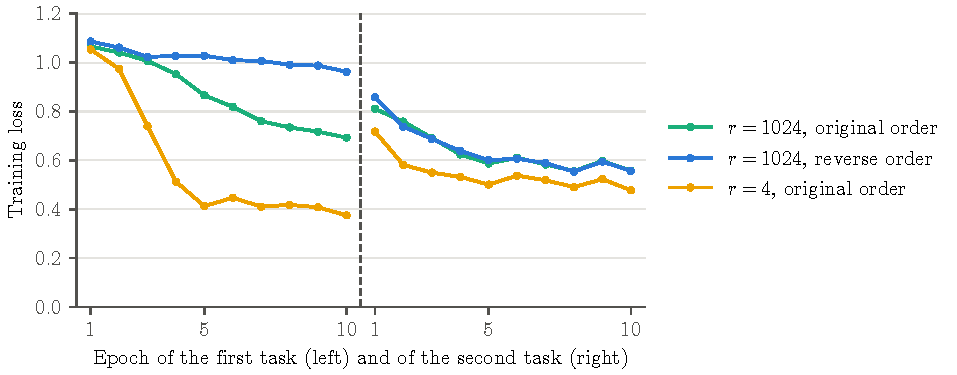
\includegraphics{figures/appA_shared_lora_loss.pdf}
% CLAUDE-DRAFT
\caption[Training loss of the first two tasks of shared LoRA]{Mean training loss per epoch of the first two tasks of shared LoRA (full training split, one run each). First task: lateral tibial cartilage in the original order, lateral meniscus in the reverse order; second task: medial tibial cartilage and medial meniscus. Dashed line: start of the second task.}
\label{fig:app-shared-loss}
\end{figure}
% source: scripts/plot_results.py (shared_lora_first_tasks_loss), run.log of tasks 1 and 2 of exp_20260926_095539_90e8b4e6 (r = 1024, original), exp_20260930_101141_5d80eb69 (r = 1024, reverse), exp_20260924_202757_88afb75d (r = 4, original)
